\documentclass[a4paper]{article}
\usepackage{graphicx}
\usepackage[utf8]{inputenc}
\usepackage{float}
\usepackage[english]{babel}
\usepackage{fancyhdr}
\usepackage[left=0.7in,top=0.9in,right=0.7in,bottom=0.9in]{geometry}
\usepackage{wrapfig}
\usepackage[english]{babel}
\usepackage{url}
\usepackage[
backend=biber
]{biblatex}
\bibliography{aaa.bib}
\usepackage{hyperref}
\usepackage{float}
\floatstyle{boxed} 

\graphicspath{/Desktop/}
\setlength{\arrayrulewidth}{0.5mm}
\setlength{\tabcolsep}{10pt}
\renewcommand{\arraystretch}{1.5}

\pagestyle{fancy}
\fancyhf{}
%\vspace{20pt}
\fancyhead[LE,RO]{Group 10  }
\fancyhead[RE,LO]{Box2d ProjectReport}
%\fancyfoot[CE,CO]{\leftmark}
\fancyfoot[LE,RO]{\thepage}


\begin{document}
	\centering
	\begin{titlepage}
	   \vspace*{\stretch{1.5}}
	   \begin{center}
	      \LARGE \textbf{Rube Goldberg Machine Simulation \\ \vspace{10pt} CS251 Box2d Project Report }\\
	      %\Large \textbf{CS215 Box2d Project Report}
	      \vspace{15mm}
			\large
	   		\begin{tabular}{ |c|c|c| }
	   			\hline
	    			Group Name & Roll No & Name \\
	   			\hline 
				 & 140050038 & Krishna \\ 	
	   			Codevita & 140050060 & Rohith \\ 
				 & 140050065 & Goutham \\ 
	   			\hline
	   		\end{tabular}
	   		\\ \vspace{15mm}
	   		\Large\textit{October 20, 2015}
	   	\end{center}
	   \vspace*{\stretch{2.5}}
	\end{titlepage}

	
	\begin{flushleft}
	\begin{itemize}
	\item{\LARGE \textbf{Motivation}}\\
	\vspace{2mm}
	\large\textit{
	Box2d makes a great general benchmark ? it?s a bottleneck on real-world apps.So we took it upon ourselves to put together a little benchmark that shows how hard can one actually perform a task which can be done in a very simple manner i.e; Goldberg Machine.So,We are using this Box2D,a 2-dimensional physics simulation engine (written in C++) to code/implement it.Every night before sleeping we put on our alarm and also will be good enough lazy to turn it off and gets irritated in the morning  as it starts buzzing.It happened to me personally when I was in a nice dream and want no one to become victim like me.This laid the foundations of our project.}
	
	
	\vspace{4mm}
	\item{\LARGE \textbf{Introduction}}\\
	\vspace{2mm}
	\large\textit{
	A \textbf{Rube Goldberg machine} is a deliberately over-engineered or overdone machine that performs a very simple task in
	a very complex fashion, usually including a chain reaction. In this project we have are going to create a simulation of a Rube
	Goldberg machine we designed, in C++ using the Box2D library.The Rube Goldberg machine?s final aim is to turn off the buzzing alarm by just pulling the thread.In this Document we have given a gist of our design, its salient features and working.}
	
	\vspace{4mm}
	\item{\LARGE \textbf{Brief Description}}\\
	\vspace{2mm}
	\large\textit{
	This section explains the original design planned in for the simulation.It reflects on the salient features of Box2D library we have utilized in our simulation and various important elements, which are a part of the simulation. The design was created without much knowledge of Box2D. So there may be a little changes in the final version.This simulatuon starts with the pendulum which is initially at its mean position and then this initiates various other simulations the wedge falls on the alarm clock and just turns it off. The only thing one must do to is to pull the thread which is attached to the pendulum and this initiates our  simulation. }
	\end{itemize}
	\end{flushleft}
	
	
	\begin{figure}[H]
	\centering
	\textit{/* Inkscape design of the silmulation*/}
	\includegraphics[width=180mm,height=95mm]{1}.
	\end{figure}
	\newpage
	
	
	
	\begin{figure}[H]
	\centering
	\vspace{20pt}
	\textit{/* Final design of the silmulation*/}
	%\vspace{20pt}
	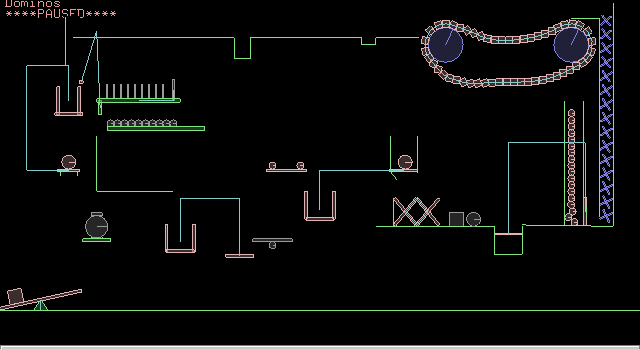
\includegraphics[width=180mm,height=95mm]{2}.
	\end{figure}
	
	\vspace{15pt}
	
	\begin{flushleft}
	\begin{itemize}
	\item{\LARGE \textbf{About Finished design of simulation}}\\
	\vspace{2mm}
	\large\textit{There is a marked variation in the originally intended design and what was finally made. First let us have a look at the differences: 
	} \\
	\begin{enumerate}
	\item \large{In the original design we had alarm clock on the floor but here we included a bit special kind of alarm which is at some height as we generally place it on a table.This alarm will be turned off as soon as we remove weight on it.This is a markable change that we had made in it.}
	
	\item \large{In the Inkscape diagram we used some curved semicircular passages through which balls traverse actually but we changed it so that these balls just noramlly fall off to the next simulative step.}
	\end{enumerate}
	\vspace{10pt}
	
	
					
				%\textit{The salient features of our simulation design which makes it unique would be as follows:}
	
	\large \textit{Now coming to the final Design, Below mentioned salient features actually makes our project unique.Here let's go and find out how these special things actually work pictorially}
	
	\section{Spring}

	\large\textit{This is actually series of X rotated by 90 degrees where this X is made of very thin rectangles.When some things gives impulse to this system, It gains horizontal momentum which inturn helps in some object moving horizontally.}
	
	\hspace{350pt} \large{(P.T.O)}
	

	\newpage
	\begin{center}
		\textit{/* Functioning of Spring*/}
	\end{center}
		\vspace{-25pt}
		\begin{figure}[H]
		\centering
		\vspace{20pt}
		%\vspace{20pt}
		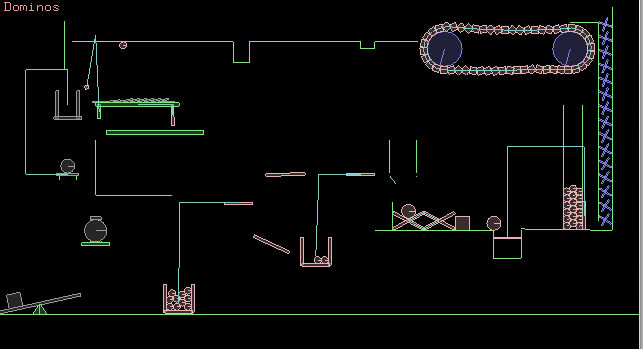
\includegraphics[width=180mm,height=95mm]{3}.
		\end{figure}
	
	\section{Balloon}
	\vspace{-10pt}
	\large\textit{We have used one balloons in the design. We used this ballon to stimulate the intermediate proceess.The balloon goes up and moves flipper. Both these balloons are Box2D circle bodies, whose gravity has been scaled to a negative value.}
			
		\vspace{10pt}
			\begin{center}
				\textit{/* Functioning of Balloon*/}
			\end{center}
		\vspace{-25pt}
		\begin{figure}[H]
		\centering
		\vspace{20pt}
		%\vspace{20pt}
		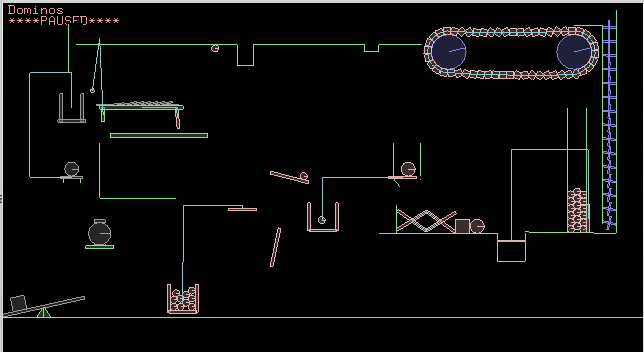
\includegraphics[width=180mm,height=95mm]{4}.
		\end{figure}
			
		\newpage
		
		\section{Rotating Vertical Lifters}
			\vspace{-10pt}
		\large\textit{Rotating vertical lifters are actually wheels which keep on rotating and helps the small shperical balls to move up through a passage kind of column on to the conveyor belt.}	
		
			\begin{center}
						\textit{/* Functioning of Vertical Lifters*/}
					\end{center}
				\vspace{-25pt}
				\begin{figure}[H]
				\centering
				\vspace{20pt}
				%\vspace{20pt}
				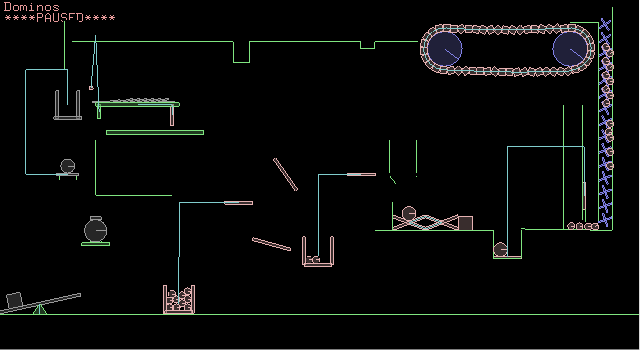
\includegraphics[width=180mm,height=90mm]{5}.
				\end{figure}
				
		\section{Conveyor Belt}
			\vspace{-10pt}
		\large\textit{The conveyor belt here actually automates the process.Here it helps help ball to move from the rotating vertical lifters to the horizontal plane.}
			\begin{center}
						\textit{/* Functioning of Conveyor Belt*/}
					\end{center}
				\vspace{-25pt}
				\begin{figure}[H]
				\centering
				\vspace{20pt}
				%\vspace{20pt}
				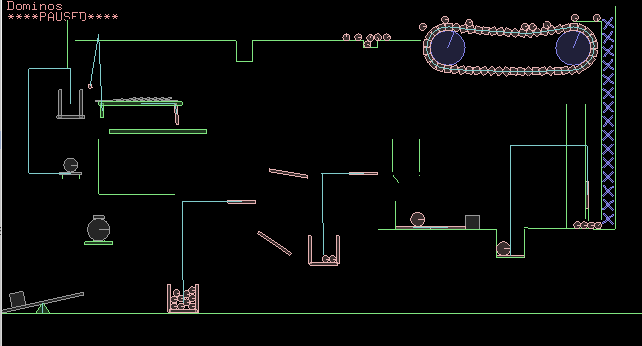
\includegraphics[width=180mm,height=90mm]{6}.
				\end{figure}
				
		\item{\LARGE \textbf{Observations regarding profiling:}}\\ 
	    \item Top 5 functions in the flat profile are:
				\begin{tabular}{ |c|c|c| }
					\hline
					percentage time & self seconds & name \\
					\hline 
					26.83 & 1.87 & b2ContactSolver::SolveTOIPositionConstraints(int,int) \\ 	
					16.50 & 1.15 & b2World::SolveTOI(b2TimeStep const\&) \\ 
					14.63 & 1.02 & b2ContactSolver::SolveVelocityConstraints() \\
		4.16 & 0.29 & b2Distance(b2DistanceOutput*, b2SimplexCache*, b2DistanceInput const*)\\
		3.59 & 0.25 &  b2World::Solve(b2TimeStep const\&) \\
					\hline
				\end{tabular}
		\item{\LARGE \textbf{Callgraph}}\\
		\begin{figure}[H]
			\centering
			\vspace{20pt}
			%\vspace{20pt}
			\includegraphics[width=180mm,height=30mm]{profile}.
		\end{figure}	
			\item{\LARGE \textbf{Work division :}}\\
			\vspace{2mm}
				\begin{tabular}{ |c|c|c| }
					\hline
					Krishna & Rohith & Goutham \\
					\hline 
				
					conveyor belt,left most pulley & rotating wheels,pulley near wheels, & spring,pulley above spring \\ 
		rotating platforms & wedge system & attatched rod near dominos \\	
		documentation & profiling & report \\
		makefile & video & webpage	\\	
					\hline
					
				\end{tabular}
				\item{\LARGE \textbf{Difficulties faced in the project:}}\\
				\large\textit{
				1.while creating the belt of conveyor belt,a problem occured joining spheres as to form a belt so we changed the spheres to rectangular boxes.\\
				2.while creating the rotating wheels to lift the spheres, a problem occured having all the wheels aligned in the same orientation initially so we changed th initial orientations of each wheel by 1 degree.
				}

	\item{\LARGE \textbf{Conclusion :}}\\
	\vspace{2mm}
	\large\textit{
	Here,we concludes about the important elements and the brief idea of our project.As this is not complete idea in terms of Box2D,we will try our level best not to change this idea much. We are also thankful to our prof.Sharath and our Guide Hitesh for helping us in this project.
	}
		\item{\LARGE \textbf{Honour code}}\\
		\large\textit{
		We pledge on our honour that we have not given or received any unauthorized assistance on this assignment or any previous task.
		}

		\end{itemize}
		
		\vspace{5pt}
		\begin{itemize}
		\item{\LARGE \textbf{References}}\\
		\end{itemize}
		\begin{enumerate}
		\item{Box2d, URL:{\url{http://www.iforce2d.net/b2dtut/}}}
		
		\item{Bibtex, URL:{\url{http://www.bibtex.org/Using/}}}
		\item{Idea from project-DharmaTeja, URL:{\url{https://www.youtube.com/watch?v=T4tV6x1vq6M}}}
		\item{Idea from Project-KaturiSaiKiran, URL:{\url{https://www.youtube.com/watch?v=rs6J7KdVKmQ}}}
		\end{enumerate}
		\end{flushleft}
		
		
	
	
	
	
	

\end{document}
